% vim:autoindent:set textwidth=78:

\section{Trabajar con datos vectoriales}\label{label_workingvector}
\index{vector layers|(}

QGIS soporta datos vectoriales en distintos formatos, incluyendo aquellos soportados por el complemento del proveedor de datos de la biblioteca OGR, tales como los archivos shape de ESRI,
\index{shapefiles}
\index{ESRI!shapefiles}
\index{SHP files}
MapInfo MIF (formato de intercambio)
\index{MIF files}
\index{MapInfo!MIF files}
y MapInfo TAB (formato nativo).
\index{TAB files}
\index{MapInfo!TAB files}
QGIS también soporta capas PostGIS
\index{PostGIS}
\index{PostgreSQL!PostGIS}
en una base de datos PostgreSQL usando el complemento del proveedor de datos PostgreSQL. Complementos de proveedores de datos adicionales proporcionan soporte para tipos de datos adicionales (ej.: texto delimitado).
\index{delimited text}

Esta sección describe cómo trabajar con dos formatos habituales: archivos shape de ESRI y capas PostGIS. Muchas de las funciones disponibles en QGIS funcionan igual cualquiera que sea la fuente de datos vectoriales. Esto es así por diseño e incluye las funciones identificar, seleccionar, etiquetar y atributos.

Trabajar con datos vectoriales de GRASS se describe en la sección \ref{sec:grass}.

\subsection{Archivos shape de ESRI}
\index{vector layers!ESRI shapefiles}
\index{shapefiles}
\index{ESRI!shapefiles}
\index{SHP files}

El soporte para archivos shape de ESRI es proporcionado por una biblioteca de funciones conocida como OGR Simple Feature Library (\url{http://www.gdal.org/ogr})\index{OGR}. Vea el Apéndice \ref{appdx_ogr} para una lista de todos los formatos soportados por OGR.

Un archivo shape en realidad consiste en al menos tres archivos:\index{shapefile!format}

\begin{itemize}
\item archivo .shp que contiene las geometrías del objeto espacial.
\item archivo .dbf que contiene los atributos en formato dBase.
\item archivo índice .shx.
\end{itemize}

Lo ideal es que haya otro archivo con extensión .prj, que contiene la información de la proyección del archivo shape.

Puede haber más archivos pertenecientes al conjunto de datos de un archivo shape. Para tener una visión más amplia sobre esto recomendamos las especificaciones técnicas del formato shape, que se pueden encontrar en \url{http://www.esri.com/library/whitepapers/pdfs/shapefile.pdf}\index{shapefile!specification}.

\subsubsection{Cargar un archivo Shape}\label{sec:load_shapefile}
{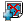
\includegraphics[width=0.7cm]{addshapefile}} Para cargar un archivo shape, arranque QGIS y haga clic en el botón \textit{Añadir una capa vectorial} de la barra de herramientas\index{shapefile!loading} o simplemente pulse la tecla "V". Esta misma herramienta se puede usar para cargar cualquiera de los formatos soportados por la biblioteca OGR. 

Al hacer clic en la herramienta aparece un diálogo estándar para abrir archivos (véase la Figura
\ref{fig:openshapefile}) que permite navegar por el sistema de archivos y cargar un archivo shape u otra fuente de datos soportada. El cuadro de selección \textsl{Archivos de tipo} permite preseleccionar algunos formatos de archivo soportados por OGR.

También puede seleccionar el tipo de codificación del archivo shape si lo desea.

\begin{figure}[h]
   \begin{center}
   \caption{Diálogo Abrir una capa vectorial soportada por OGR}\label{fig:openshapefile}\smallskip
   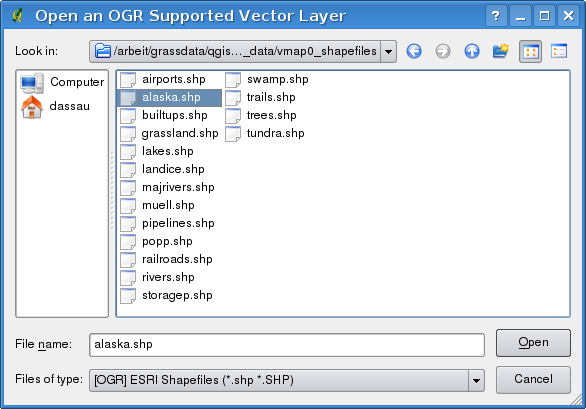
\includegraphics[clip=true, width=14cm]{shapefileopendialog}
\end{center} 
\end{figure}

Al seleccionar un archivo shape de la lista y hacer clic en Abrir, éste se carga en QGIS. La Figura
\ref{fig:loadedshapefile} muestra QGIS después de cargar el archivo alaska.shp.

\begin{figure}[ht]
   \begin{center}
   \caption{QGIS con el archivo Shape de Alaska cargado}\label{fig:loadedshapefile}\smallskip
   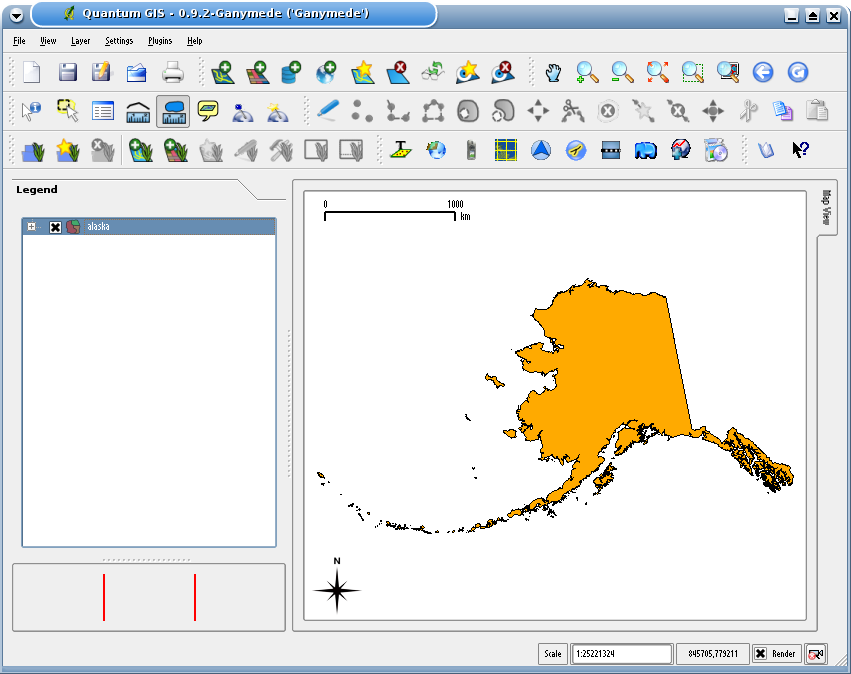
\includegraphics[clip=true, width=17cm]{shapefileloaded09}
\end{center} 
\end{figure}

\begin{Tip}\caption{\textsc{Colores de capas}}
\qgistip{Cuando añade una capa al mapa, se le asigna un color aleatorio. Cuando se añade más de una capa a la vez, se asignan colores diferentes a cada una. }
\end{Tip}

Una vez cargada, se puede desplazar por el archivo shape usando las herramientas de navegación del mapa. Para cambiar la simbología de una capa, abra el diálogo de propiedades de la capa haciendo doble clic en el nombre de la capa en la leyenda o clic derecho y seleccionando \textsl{Propiedades} del menú emergente. Vea la Sección \ref{sec:symbology} para más información sobre la configuración de la simbología de capas vectoriales.
  
\subsubsection{Mejorar el rendimiento}

Para mejorar el rendimiento al dibujar un archivo shape, puede crear un índice espacial. Un índice espacial \index{spatial index!shapefiles} mejorará la velocidad tanto al hacer zum como al desplazar la capa. Los índices espaciales usados por QGIS tienen la extensión \textsl{.qix}.

Siga estos pasos para crear el índice:

\begin{itemize}
\item Cargue un archivo shape.
\item Abra el diálogo \textit{Propiedades de la capa} haciendo doble clic en el nombre del archivo shape en la leyenda o mediante clic derecho y eligiendo \textit{Propiedades} en el menú emergente.
\item En la pestaña \textit{General} haga clic en el botón \textit{Crear} en el recuadro \textit{Índice espacial}.
\end{itemize}

\subsubsection{Cargar una capa MapInfo}
\index{vector layers!MapInfo}

Para cargar una capa MapInfo, haga clic en el botón \textit{Añadir una capa vectorial} de la barra de herramientas o pulse la tecla "V", cambie el filtro de tipo de archivo a \textit{MapInfo (*.mif *.tab *.MIF *.TAB)} y seleccione la capa que quiere cargar.

\subsubsection{Cargar una cobertura de ArcInfo}
\index{vector layers!ArcInfo Coverage}

Cargar una cobertura de ArcInfo se hace usando el mismo método que para archivos shape o capas MapInfo. Haga clic en el botón \textit{Añadir una capa vectorial} de la barra de herramientas o pulse la tecla "V" para abrir el diálogo y cambie el filtro de tipo de archivo a \textit{Todos los archivos (*.*)}. Navegue al directorio de coberturas y elija uno de los siguientes archivos (si están presentes en su cobertura):

\begin{itemize}
\item .lab - para cargar una capa de etiquetas (etiquetas de polígonos o puntos fijos).
\item .cnt - para cargar una capa de centroides de polígono.
\item .arc - para cargar una capa arc (línea).
\item .pal - para cargar una capa de polígonos.
\end{itemize}

\subsection{Capas PostGIS}
\index{vector layers!PostGIS|see{PostGIS}}
\index{PostGIS!layers}
\label{label_postgis} 

Las capas PostGIS se guardan en una base de datos PostgreSQL. Las ventajas de PostGIS son el indexado espacial, filtrado y capacidad de consulta. Usar las funciones vectoriales de PostGIS, tales como seleccionar e identificar, es más preciso que con otras capas en QGIS.

Para usar capas PostGIS debe:\index{PostgreSQL!loading layers}

\begin{itemize}
\item Crear una conexión guardada en QGIS a la base de datos PostgreSQL (si no hay ya una definida).\index{PostgreSQL!connection}
\item Conectarse a la base de datos.
\item Seleccionar la capa a añadir al mapa.
\item Opcionalmente, proporcionar una sentencia SQL \textit{where} para definir qué objetos espaciales cargar de la capa.
\item Cargar la capa.
\end{itemize}

\subsubsection{Crear una conexión guardada}\index{PostgreSQL!connection}\label{sec:postgis_stored}

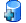
\includegraphics[width=0.7cm]{addpostgis} La primera vez que use una fuente de datos PostGIS, debe crear una conexión a la base de datos PostgreSQL que contenga los datos. Empiece por hacer clic en el botón \textit{Añadir una capa de PostGIS} de la barra de herramientas, seleccionar la opción \textit{Añadir una capa de PostGIS...} del menú \textit{Capa} o pulsar la tecla "D". Se mostrará el diálogo \textsl{Añadir tabla(s) PostGIS}. Para acceder al administrador de conexiones\index{PostgreSQL!connection
manager}, pulse el botón \textsl{Nueva} para mostrar el diálogo \textsl{Crear una nueva conexión a PostGIS}. Las parámetros requeridos para una conexión se muestran en la Tabla \ref{tab:postgis_connection_parms}.

\begin{table}[h]\index{PostgreSQL!connection parameters}
\centering
\caption{Parámetros de conexión PostGIS}\label{tab:postgis_connection_parms}\medskip
 \begin{tabular}{|l|p{5in}|}
\hline Nombre & Un nombre para esta conexión. Puede ser el mismo que el de la \textsl{Base de datos}.
\\
\hline Servidor \index{PostgreSQL!host}
& Nombre del servidor de la base de datos. Debe ser un nombre de servidor que se pueda resolver, lo mismo que si fuera a ser usado para abrir una conexión telnet o hacer ping al servidor. \\
\hline Base de datos \index{PostgreSQL!database} & Nombre de la base de datos.  \\
\hline Puerto \index{PostgreSQL!port}& Número del puerto al que responde el servidor de la base de datos PostgreSQL. El puerto predeterminado es 5432.\\
\hline Nombre de usuario \index{PostgreSQL!username}& Nombre de usuario utilizado para conectarse a la base da datos. \\
\hline Contraseña \index{PostgreSQL!password}& Contraseña usada con el \textsl{Nombre de usuario} para conectarse a la base de datos.\\
\hline
\end{tabular}
\end{table}

Una vez que se han rellenado los parámetros, puede probar la conexión pulsando en el botón \textsl{Probar conexión}\index{PostgreSQL!connection!testing}. Para guardar la contraseña con la información de la conexión, marque la opción \textsl{Guardar contraseña}.

\begin{Tip}\caption{\textsc{Configuración de usuario de QGIS y seguridad}}\index{settings}\index{security}
\qgistip{Su configuración personal para QGIS se guarda en base al sistema operativo. En Linux/Unix, la configuración se guarda en su directorio personal en .qt/qgisrc. En Windows, la configuración se guarda en el registro. Dependiendo de su entorno de procesamiento, guardar contraseñas en su configuración de QGIS puede ser un riesgo de seguridad.
}
\end{Tip}

\subsubsection{Cargar una capa PostGIS}\index{PostgreSQL!loading layers}

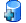
\includegraphics[width=0.7cm]{addpostgis} Una vez que tiene una o más conexiones definidas, puede cargar capas de la base de datos PostgreSQL. Por supuesto, esto requiere tener datos en PostgreSQL. Vea la Sección \ref{sec:loading_postgis_data} donde se trata la importación de datos a la base de datos. 

Para cargar una capa desde PostGIS, realice los siguientes pasos:

\begin{itemize}
\item Si el diálogo de capas PostGIS no está aún abierto, pulse el botón \textit{Añadir una capa de PostGIS} de la barra de herramientas.
\item Seleccione la conexión de la lista desplegable y pulse \textsl{Conectar}.
\item Encuentre la capa que desee añadir en la lista de capas disponibles.
\item Selecciónela haciendo clic en ella. Puede seleccionar múltiples capas manteniendo pulsada la tecla Mayúsculas a la vez que hace clic. Vea la Sección \ref{sec:query_builder} para información sobre el uso del constructor de consultas de PostgreSQL para definir mejor la capa.
\item Haga clic en el botón \textsl{Añadir} para añadir la capa al mapa.
\end{itemize}

\begin{Tip}\caption{\textsc{Capas PostGIS}}
\qgistip{Normalmente una capa PostGIS está definida pur una entrada en la tabla geometry\_columns. Desde la versión \OLD en adelante, QGIS puede cargar capas que no tienen una entrada en la tabla geometry\_columns. Esto incluye tanto tablas como vistas. Definir una vista espacial proporciona un método potente de visualizar sus datos. Consulte su manual de PostgreSQL para información sobre la creación de vistas.}
\end{Tip}

\subsubsection{Algunos detalles sobre las capas PostgreSQL}\label{sec:postgis_details}
\index{PostgreSQL!layer details}

Esta sección contiene algunos detalles sobre cómo accede QGIS a capas PostgreSQL. La mayoría de las veces QGIS debería simplemente proporcionarle una lista de tablas de base de datos que puede cargar y cargarlas según se le pida. Sin embargo, si tiene problemas para cargar una tabla de PostgreSQL en QGIS, la información que sigue le puede ayudar a entender cualquier mensaje de QGIS y darle una dirección en la que cambiar la tabla de PostgreSQL o la definición de la vista para permitir que QGIS la cargue.

QGIS requiere que las capas PostgreSQL contengan una columna que se pueda usar como clave única para la capa. Esto normalmente significa que la tabla necesita una clave primaria o tener una columna con una restricción única en ella. QGIS además necesita que esta columna sea de tipo int4 (un entero con un tamaño de 4 bytes). Si una tabla carece de estos elementos, la columna oid se usará en su lugar. Las prestaciones mejorarán si la columna está indexada (tenga en cuenta que las claves primarias se indexan automáticamente en PostgreSQL).

Si la capa PostgreSQL es una vista existen los mismos requisitos, pero las vistas no tienen claves primarias o columnas con restricciones únicas. En este caso QGIS intentará encontrar una columna en la vista que sea derivada de una columna de la tabla que sea adecuada. Si no se puede encontrar una, QGIS no cargará la capa. Si ocurre esto, la solución es modificar la vista para que incluya una columna adecuada (de tipo int4 y una clave primaria o con una restricción única, preferiblemente indexada).

\subsubsection{Importar datos a PostgreSQL}\label{sec:loading_postgis_data}
\index{PostGIS!SPIT!importing data}

\minisec{shp2pgsql}
Se pueden importar datos a PostgreSQL usando distintos métodos. PostGIS incluye una utilidad llamada \textsl{shp2pgsql} que se puede usar para importar archivos shape a bases de datos activadas PostGIS. Por ejemplo, para importar un archivo shape llamado lagos a una base de datos PostgreSQL llamada datos\_sig, use el siguietne comando:

\begin{verbatim} 
  shp2pgsql -s 2964 lagos.shp lagos_nueva | psql datos_sig
\end{verbatim}

Esto crea una nueva capa llamada lago\_nueva en la base de datos datos\_sig. La nueva capa tendrá el mismo identificador de referencia espacial (SRID) de 2964. Vea la Sección \ref{label_projections} para más información sobre los sistemas de referencia espacial y las proyecciones.
\begin{Tip}
\caption{\textsc{Exportar conjuntos de datos de PostGIS}\index{PostGIS!Exporting}}
\qgistip{Al igual que la herramienta de importación \textsl{shp2pgsql} también hay una herramienta para exportar conjuntos de datos PostGIS a archivos shape: \textsl{pgsql2shp}. Ésta está incluida e su distribución PostGIS.}
\end{Tip}

\minisec{Complemento SPIT}

\includegraphics[width=0.7cm]{spiticon} QGIS viene con un complemento llamado SPIT (Shapefile to PostGIS Import Tool->Herramienta de Importación de Archivos Shape a PostGIS)\index{PostGIS!SPIT}. SPIT se puede usar para cargar múltiples archivos shape al mismo tiempo e incluye soporte para esquemas. Para usar SPIT, abra el Administrador de complementos desde el menú \textit{Complementos}, marque la casilla junto al complemento SPIT y pulse Aceptar. El icono de SPIT se añadirá a la barra de herramientas de complementos\index{PostGIS!SPIT!loading}.

Para importar un archivo shape, haga clic en la herramienta SPIT en la barra de herramientas para abrir el diálogo. Puede añadir uno o más archivos a la cola haciendo clic en el botón \textsl{Añadir}. Para procesar los archivos, haga clic  en el botón \textsl{Importar}. El progreso de la importación y cualquier error/aviso se mostrará a medida que se procesa cada archivo shape.

\begin{Tip}\caption{\textsc{Importar archivos shape que contienen palabras reservadas de PostgreSQL}}\index{PostGIS!SPIT!reserved words}
\qgistip{Si se añade un archivo shape a la cola que contiene campos que son palabras reservadas en una base de datos PostgreSQL aparecerá un diálogo mostrando el estado de cada campo. Puede editar los nombre de los campos\index{PostGIS!SPIT!editing field names} antes de importar y cambiar aquellos que sean palabras reservadas (o cambiar cualquier otro nombre de campo si lo desea). Intentar importar un archivo shape con palabras reservadas como nombres de campos probablemente fallará.}
\end{Tip} 

\minisec{ogr2ogr}
Además de \textit{shp2pgsql} y \textit{SPIT} hay otra herramienta para suministrar datos en PostGIS: \textit{ogr2ogr}. Esto es parte de su instalación de GDAL. Para importar un archivo shape a PostGIS, haga lo siguiente:
\begin{verbatim}
  ogr2ogr -f "PostgreSQL" PG:"dbname=postgis host=myhost.de user=postgres \
  password=topsecret" alaska.shp
\end{verbatim}

Esto importará el archivo shape alaska.shp a la base de datos PostGIS \textit{postgis} usando el usuario \textit{postgres} con la contraseña \textit{topsecret} en el servidor
\textit{myhost.de}.

Tenga en cuenta que OGR debe estar compilado contra PostgreSQL para soportar PostGIS. Puede ver esto tecleando
\begin{verbatim}
ogrinfo --formats | grep -i post
\end{verbatim}

\subsubsection{Mejorar el rendimiento}\label{label_improve}

Recuperar objetos espaciales de una base de datos PostgreSQL puede llevar tiempo, especialmente a través de una red. Puede mejorar el rendimiento al dibujar capas de PostgreSQL asegurándose de que existe un índice espacial \index{PostGIS!spatial index} para cada capa de la base de datos. PostGIS soporta la creación de un \index{PostGIS!spatial index!GiST} índice GiST (Generalized Search Tree->Árbol de búsqueda generalizado) para acelerar las búsquedas espaciales de los datos.

La sintaxis para crear un índice GiST\footnote{La información de los índices GiST se ha tomado de la documentación de PostGIS disponible en http://postgis.refractions.net} es:

\begin{verbatim}
    CREATE INDEX [nombreindice] ON [nombretabla] 
      USING GIST ( [campogeometria] GIST_GEOMETRY_OPS );
\end{verbatim}

Tenga en cuenta que para grandes tablas, la creación del índice puede llevar bastante tiempo. Una vez que se ha creado el índice, se debería realizar un \textit{VACUUM ANALYZE}. Vea la documentación de PostGIS \cite{PostGISweb} para más información.

El siguiente es un ejemplo de la creación de un índice GiST:
\begin{verbatim}
gsherman@madison:~/current$ psql gis_data
Welcome to psql 8.0.0, the PostgreSQL interactive terminal.

Type:  \copyright for distribution terms
        \h for help with SQL commands
        \? for help with psql commands
        \g or terminate with semicolon to execute query
        \q to quit

gis_data=# CREATE INDEX sidx_lagos_alaska ON lagos_alaska
gis_data-# USING GIST (la_geometria GIST_GEOMETRY_OPS);
CREATE INDEX
gis_data=# VACUUM ANALYZE lagos_alaska;
VACUUM
gis_data=# \q
gsherman@madison:~/current$
\end{verbatim}

\subsection{El diálogo Propiedades de la capa}\label{sec:vectorprops}
\index{vector layers!properties dialog}

El diálogo de propiedades de las capas vectoriales proporciona información sobre una capa, configuración de la simbología y opciones de etiquetado. Si su capa vectorial se ha cargado desde un almacén PostgreSQL / PostGIS, también puede modificar la consulta SQL subyacente para la capa - bien a mano, editando la SQL en la pestaña \textit{General} o invocando el diálogo \textit{Constructor de consultas} en la pestaña \textit{General}. Para acceder al diálogo \textit{Propiedades de la capa}, haga doble clic en una capa en la leyenda o clic derecho en la capa y seleccione \textit{Propiedades} del menú emergente.

\subsubsection{Pestaña Simbología}\label{sec:symbology}
\index{vector layers!symbology}

QGIS soporta varios trazadores de simbología para controlar cómo se muestran los objetos espaciales vectoriales. Actualmente están disponibles los siguientes trazadores:

\begin{description}
    \item[Símbolo único] - se aplica un solo estilo a cada objeto de la capa.\index{vector layers!renderers!single symbol}
    \item[Símbolo graduado] - los objetos de la capa se muestran con diferentes símbolos clasificados por los valores de un campo particular.\index{vector layers!renderers!graduated symbol}
    \item[Color contínuo] - los objetos de la capa se muestran con un abanico de colores clasificados por el valor numérico de un campo especificado.\index{vector layers!renderers!continuous
color}
    \item[Valor único] - los objetos se clasifican por el valor único contenido en un campo especificado, teniendo cada valor un símbolo diferente.\index{vector layers!renderers!unique value}
\end{description}

Para cambiar la simbología de una capa, simplemente haga doble clic en su entrada en la leyenda y se mostrará el diálogo \textit{Propiedades de la capa}.\index{symbology!changing}.

\begin{figure}[H]
   \begin{center}
   \caption{Diálogo Propiedades de la capa}\label{fig:vector_symbology}\smallskip
   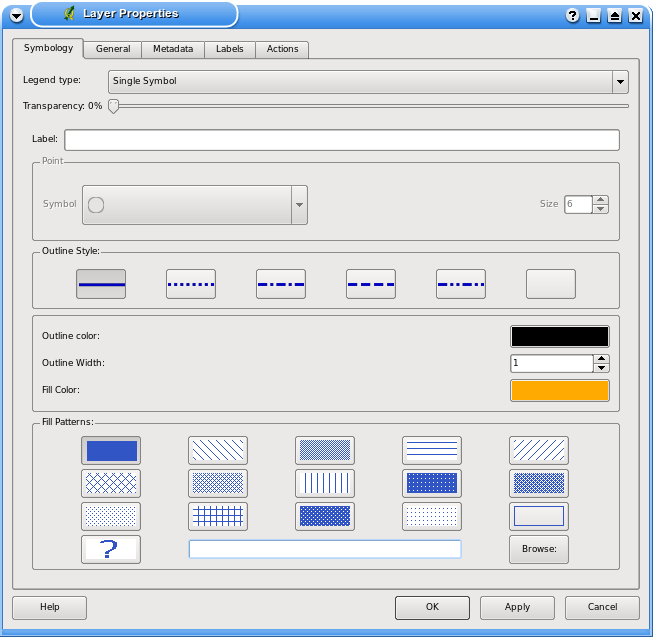
\includegraphics[clip=true, width=14cm]{vectorLayerSymbology09} 
\end{center}  
\end{figure}

\textbf{Nuevo en v0.9} hay una funcion para usar archivos de imagen guardados en su equipo como patrón de relleno de capas vectoriales.

\minisec{Transparencia de vectoriales} \label{sec:vect_transparency} \index{vector layers!transparency}
QGIS \CURRENT permite establecer una transparencia para cada capa vectorial. Esto se puede hacer con del deslizador que hay justo debajo del tipo de leyenda (ver fig. \ref{fig:vector_symbology}). Esto es muy útil para superponer varias capas vectoriales.

\subsubsection{Pestaña General}
La pestaña General es muy similar a la del diálogo de capas ráster. Permite cambiar el nombre que se muestra, establecer opciones de visualización dependientes de la escala, crear un índice espacial del archivo vectorial (sóĺo para formatos soportados por OGR y PostGIS) y ver o cambiar la proyección.

El botón \textsl{Constructor de consultas} permite crear un subconjunto de los objetos espaciales de la capa - pero este botón actualmente sólo esta disponible cuando abre la tabla de atributos y selecciona el botón \textsl{Avanzado...}.

\subsubsection{Pestaña Metadatos}

La pestaña metadatos contiene información sobre la capa, incluyendo especificaciones sobre el tipo y la localización, número de objetos espaciales, tipo de objetos espaciales y las posibilidades de edición. Los campos proyección y atributos y sus tipos de datos se muestran en esta pestaña. Esta es una manera rápida de obtener información sobre la capa.

\subsubsection{Pestaña Etiquetas}

La pestaña etiquetas le permite activar el etiquetado de los objetos espaciales y controlar varias opciones relacionadas con el emplazamiento, estilo y márgenes.

Ilustraremos esto etiquetando el archivo shape lagos de los datos de ejemplo de qgis:

\begin{enumerate}
\item Cargue los archivos shape alaska.shp y lagos.shp en QGIS.
\item Acerque el zum un poco a su zona favorita con algunos lagos.
\item Haga la capa \textsl{lagos} activa.
\item Abra el diálogo de propiedades.
\item Pulse en la pestaña ``Etiquetas''.
\item Marque la casilla ``Mostrar etiquetas'' para activar el etiquetado.
\item Seleccione el campo con el que etiquetar. Usaremos \textsl{NAMES}.
\item Introduzca una etiqueta predeterminada para los lagos que no tienen nombre. La etiqueta predeterminada se usará cada vez que QGIS encuentre un lago sin valor en el campo \textsl{NAMES}.
\item Pulse \textsl{Aplicar}.
\end{enumerate} 

Ahora tenemos etiquetas. ¿Qué aspecto tienen? Probablemente son demasiado grandes o están mal situadas en relación con el símbolo marcador para los lagos.

Haga clic en la pestaña ``Estilo de fuente'' y use los botones \textsl{Fuente} y \textsl{Color} para establecer la fuente y el color.

Para cambiar la posición de la fuente en relación con el objeto espacial:

\begin{enumerate} 
\item Haga clic en la pestaña ``Alineación de fuente''.
\item Cambie la ubicación seleccionando uno de los botones circulares en el grupo ``Ubicación''. Para colocar nuestras etiquetas, seleccione el botón circular ``Derecha''.
\item Pulse \textsl{Aplicar} para ver sus cambios sin cerrar el diálogo.
\end{enumerate} 

Va mejorando, pero las etiquetas todavía están demasiado cerca del marcador. Para solucionarlo, podemos usar las opciones de la pestaña ``Posición''. Aquí podemos añadir desplazamientos en las direcciones X e Y. Añadir un desplazamiento 5 en la X separará nuestras etiquetas del marcador y las hará más legibles. Por supuesto, si el símbolo o la fuente de su marcador son mayores, se requerirá un desplazamiento mayor.

El último ajuste que haremos será poner un márgen a las etiquetas. Esto simplemente significa poner un fondo alrededor de las etiquetas para que destaquen más. Para poner un margen a las etiquetas de los lagos:

\begin{enumerate}
\item Pulse la pestaña ``Margen''.
\item Marque la casilla ``¿Poner margen a las etiquetas?'' para activar los márgenes.
\item Seleccione un tamaño para el margen usando las flechas del cuadro tamaño.
\item Seleccione un color pulsando el botón \textsl{Color} y eligiendo su color favorito del selector de colores.
\item Haga clic en \textsl{Aplicar} para ver si le gustan los cambios.
\end{enumerate} 

Si no está conforme con los resultados, cambie los ajustes y pruebe otra vez pulsando \textsl{Aplicar}.

Un margen de 2 puntos parece dar buen resultado. Tenga en cuenta que también puede especificar el tamaño del margen en unidades del mapa si eso le conviene más.

El resto de las pestañas en la pestaña ``Etiquetas'' la permiten controlar el aspecto de las etiquetas usando atributos guardados en la capa. Las pestañas ``Datos'' le permiten establecer todos los parámetros de las etiquetas usando campos de la capa.

\subsubsection{Pestaña Acciones}\index{actions}\label{label_actions}

QGIS proporciona la capacidad de realizar una acción en base a los atributos de un objeto espacial. Esto se puede usar para realizar cualquier número de acciones, por ejemplo, ejecutar un programa con argumentos elaborados a partir de los atributos de un objeto espacial o pasando parámetros a una herramienta de informes vía web.

Las acciones son útiles cuando con frecuencia se quiere ejecutar una aplicación externa o ver una página web basada en uno o más valores de su capa vectorial. Un ejemplo es realizar una búsqueda basada en el valor de un atributo. Este concepto se usa en la siguiente explicación.

\minisec{Definir acciones}\index{actions!defining}

Las acciones de atributos se definen desde el diálogo de propiedades de capas vectoriales. Para definir una acción, abra el diálogo de propiedades de capas vectoriales y pulse la pestaña \textit{Acciones}. Proporcione un nombre descriptivo para la acción. La propia acción debe contener el nombre de la aplicación que se ejecutará cuando se la invoque. Puede añadir uno o más valores de campos de atributos como argumentos para la aplicación. Cuando se invoca la acción cualquier conjunto de caracteres que empiece con un \% seguido por el nombre de un campo se reemplazará por el valor de ese campo. Los caracteres especiales \%\% \index{\%\%}se sustituirán por el valor del campo que se seleccionó en los resultados de la identificación o en la tabla de atributos (vea Usar acciones más abajo). Las comillas dobles se pueden usar para agrupor texto en un solo argumento para el programa, script o comando. Las comillas dobles se ignorarán si van precedidas de una barra invertida.

A continuación se muestran dos ejemplos:\index{actions!examples}

\begin{itemize}
  \item \texttt{konqueror http://www.google.com/search?q=\%nam}
  \item \texttt{konqueror http://www.google.com/search?q=\%\%}
\end{itemize}


En el primer ejemplo, se invoca al navegador web konqueror y se le pasa una URL para que la abra. La URL realiza una búsqueda en Google con el valor del campo \textit{nam} de nuestra capa vectorial. Tenga en cuenta que la aplicación o script llamado por la acción debe estar en su variable de entorno PATH o si no debe proporcionar la ruta completa. Para asegurarse, podríamos rescribir el primer ejemplo como: \texttt{/opt/kde3/bin/konqueror
http://www.google.com/search?q=\%nam}. Esto asegurará que la aplicación konqueror se ejecute cuando se invoque la acción.

El segundo ejemplo usa la notación \%\% que no recae en un campo particular para su valor. Cuando se invoca la acción, \%\% será reemplazado por el valor del campo seleccionado en los resultados de la identificación o en la tabla de atributos.

\minisec{Usar acciones}\index{actions!using}\label{label_usingactions}

Se pueden invocar las acciones tanto desde el diálogo \textit{Resultados de la identificación} como desde el diálogo \textit{Tabla de atributos}. Para invocar una acción, haga clic derecho en el registro y seleccione la acción del menú emergente. Las acciones se listan en el menú emergente por el nombre que les asignó al definir las acciones. Pulse en la acción que quiera invocar.

Si está invocando una acción que usa la notación \%\%, haga clic derecho en el valor del campo que quiera pasar a la aplicación o script en el diálogo \textit{Resultados de la identificación} o en el diálogo \textit{Tabla de atributos}.

Aquí hay otro ejemplo que extrae datos de una capa vectorial y los inserta en un archivo usando bash y el comando `echo' (así que sólo funcionará en GNU/Linux y quizás en Mac OS X). La capa en cuestión tiene campos para el nombre de una especie (taxon\_name), la latitud (lat) y la longitud (long). Me gustaría poder hacer una selección espacial de unas localizaciones y exportar los valores de esos campos de los registros seleccionados (mostrados en amarillo en el área del mapa de QGIS) a un archivo de texto. Aquí está la acción para llevar esto a cabo:

\begin{verbatim}
  bash -c "echo \"%taxon_name %lat %long\" >> /tmp/species_localities.txt"
\end{verbatim} 

Después de seleccionar unas cuantas localizaciones y ejecutar la acción en cada una de ellas, al abrir el archivo de salida se mostrará algo parecido a esto:

\begin{verbatim}
  Acacia mearnsii -34.0800000000 150.0800000000
  Acacia mearnsii -34.9000000000 150.1200000000
  Acacia mearnsii -35.2200000000 149.9300000000
  Acacia mearnsii -32.2700000000 150.4100000000
\end{verbatim} 

Como ejercicio podemos crear una acción que haga una búsqueda en Google sobre la capa \textsl{lagos}. Primero necesitamos determiar la URL que hace falta para realizar la búsqueda sobre una palabra clave. Esto se hace fácilmente simplemente yendo a Google, haciendo una búsqueda sencilla y tomando la URL de la barra de direcciones del navegador. Con este pequeño esfuerzo vemos que el formato es: \url{http://google.com/search?q=qgis}, donde \textit{qgis} es el término de búsqueda. Con esta información podemos continuar:

\begin{itemize}
\item Asegúrese de que la capa \textsl{lagos} está cargada.
\item Abra el diálogo de propiedades haciendo doble clic en la capa en la leyenda o clic derecho y seleccionando \textsl{Propiedades} del menú emergente.
\item Haga clic en la pestaña ``Acciones''.
\item Introduzca un nombre para la acción, por ejemplo ``Búsqueda Google''.
\item Para la acción, necesitamos proporcionar el nombre de un programa externo a ejecutar. En este caso, podemos usar Firefox. Si el programa no está en su variable de entorno PATH, tiene que proporcionar la ruta completa.
\item A continuación del nombre de la aplicación externa, añada la URL usada para hacer la búsqueda en Google, sin incluir el término de búsqueda:
  \url{http://google.com/search?q=}
\item El texto en el campo ``Acción'' debería ser como este:\\
  \texttt{firefox http://google.com/search?q=}
\item Haga clic en el cuadro desplegable que contiene los nombre de los campos de la capa \textsl{lagos}. Se encuentra a la derecha del botón \textsl{Insertar campo}.
\item Del cuadro desplegable, seleccione \textsl{NAMES} y haga clic en \textsl{Insertar campo}
\item El texto de su acción ahora tiene este aspecto:\\ \texttt{firefox http://google.com/search?q=\%NAMES}
\end{itemize}
 
Esto completa la acción que ya está lista para usar. El texto final de la acción debería ser como este:

\begin{center}
\texttt{firefox http://google.com/search?q=\%NAMES}
\end{center}

Ahora podemos usar la acción. Cierre el diálogo de propiedades y acerque el zum a un área de su interés. Asegúrese de que la capa \textsl{lagos} está activa e identifique un lago. En el cuadro de resultados verá ahora visible nuestra acción:

\begin{figure}[H]
   \begin{center}
   \caption{Seleccionar objeto espacial y elegir acción}\label{fig:identify_action}\smallskip
   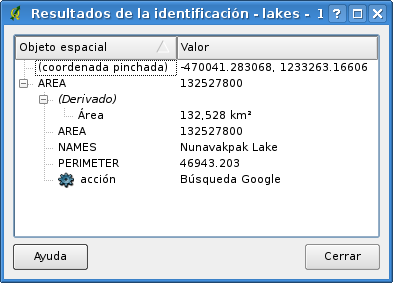
\includegraphics[clip=true, width=8cm]{identify_action} 
\end{center}
\end{figure}

Cuando pulsamos sobre la acción, ésta abre Firefox y navega hasta la URL
\url{http://www.google.com/search?q=Tustumena}. También es posible añadir más campos de atributos a la acción. Para ello puede añadir un ``+'' al final del texto de la acción, seleccionar otro campo y pulsar en \textsl{Insertar campo}. En este ejemplo no hay ningún otro campo disponible en el que tuviera sentido buscar.

Puede definir múltiples acciones para una capa y cada una aparecerá en el diálogo Resultados de la identificación. También puede invocar las acciones desde la tabla de atributos, seleccionando una fila, haciendo clic derecho y luego eligiendo la acción del menú emergente.

Se le pueden ocurrir toda clase de usos para las acciones. Por ejemplo, si tiene una capa de puntos que contiene localizaciones de imágenes o fotos junto con un nombre de archivo, podría crear una acción para lanzar un visor para mostrar la imagen. También podría usar las acciones para lanzar informes basados en web para un campo de atributos o combinación de campos, especificándolos de la misma forma que lo hicimos para nuestro ejemplo de búsqueda en Google.

\subsection{Edición}\index{editing}

QGIS soporta capacidades básicas de edición de datos espaciales. Antes de continuar leyendo, debería tener en cuenta que en este nivel de desarrollo el soporte de edición todavía es preliminar. Antes de hacer cualquier edición, haga siempre una copia de respaldo de los datos que vaya a editar.

\textbf{Nota} – el procedimiento para editar capas de GRASS es diferente – vea la Sección \ref{grass_digitising} para más detalles.

\subsubsection{Establecer la tolerancia de autoensamblado}

Antes de poder editar vértices, necesitamos establecer la tolerancia de autoensamblado. Ésta es la distancia que QGIS utilizar para ``buscar'' el polígono y vértice que está intentando editar cuando pulsa en el mapa. Si no se encuentra dentro de la tolerancia de autoensamblado, QIGS no encontrará ni seleccionará el vértice para editarlo. La tolerancia se establece en las unidades del mapa, por lo que puede necesitar experimentar hasta conseguir establecerla correctamente. Si especifica una tolerancia excesiva, QGIS se puede autoensamblar al vértice incorrecto, especialmente si está trabajando con un gran número de vértices que se encuentran próximos. Si establece una tolerancia demasiado pequeña no encontrará nada y aparecerá un molesto aviso a tal efecto.

Para establecer la tolerancia de autoensamblado, seleccione \textsl{Propiedades del proyecto} del menú \textsl{Configuración} y pulse en la pestaña ``General''.  Recuerde que la tolerancia está en unidades de mapa. Para nuestro pequeño proyecto de digitalización, las unidades están en grados decimales. Sus resultados pueden variar, pero algo del orden de 0.05 a 0.1 debería ir bien.

\subsubsection{Editar una capa existente}
\index{vector layers!editing}
\index{editing!an existing layer}
\label{sec:edit_existing_layer}

De forma predeterminada, QGIS carga las capas en modo de sólo lectura: esto es una medida de seguridad para evitar que se edite una capa de forma accidental si hay un descuido con el ratón. Sin embargo, puede seleccionar para editar cualquier capa con tal de que el proveedor de los datos tenga soporte para ella y la fuente de datos subyacente se pueda escribir (esto es, sus archivos no sean de sólo lectura).

La edición de capas en más versátil cuando se usa sobre fuentes de datos PostgreSQL/PostGIS.

\begin{Tip}[h]\caption{\textsc{Integridad de los datos}}
\qgistip{Por favor, considere hacer una copia de respaldo de sus datos originales antes de empezar a editar y también a intervalos regulares durante la edición. QGIS está todavía en estado de pre-versión 1.0 y por lo tanto puede que no sea capaz de proteger sus datos en todas las situaciones.
}
\end{Tip}

\index{Allow Editing}
Todas las sesiones de edición comienzan al seleccionar la opción \textit{Conmutar edición}. Esta opción se puede encontrar en el menú emergente después de hacer clic derecho en la entrada de la leyenda para esa capa. De forma alternativa, puede usar el botón \index{Toggle Editing} 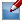
\includegraphics[width=0.4cm, clip=true]{StartEditing} 
\textit{Conmutar edición} de la barra de herramientas para iniciar o parar el modo de edición.\index{editing!icons}

\begin{Tip}[h]\caption{\textsc{Editar un mapa es distinto de editar una tabla de atributos}}
\qgistip{En esta versión de QGIS, el binomio \textit{Iniciar edición}/\textit{Detener edición} sobre la vista del mapa funciona por separado del binomio \textit{Iniciar edición}/\textit{Detener edición} en una tabla de atributos.
}
\end{Tip}

\begin{Tip}[h]\caption{\textsc{Guardar regularmente}}
\qgistip{Recuerde desactivar \textit{Conmutar edición} o seleccionar el botón \textit{Detener edición} regularmente. Esto permite guardar sus cambios hechos hasta ese momento y también confirma que su fuente de datos puede admitir todos sus cambios.
}
\end{Tip}

\begin{Tip}[h]\caption{\textsc{Ediciones concurrentes}}
\qgistip{Esta versión de QGIS no controla si alguien más está editando un objeto espacial al mismo tiempo que usted. El último editor gana.
}
\end{Tip}

Una vez que la capa está en modo de edición, aparecerán marcadores en los vértices.

\begin{Tip}[h]\caption{\textsc{Acercar zum antes de editar}}
\qgistip{Antes de editar una capa, debería acercar el zum a su área de interés. Esto evita tener que esperar mientras todos los marcadores de vértices son representados a lo largo de toda la capa.
}
\end{Tip}

\begin{Tip}[h]\caption{\textsc{Marcadores de vértices}}
\qgistip{Esta versión de QGIS no le permite cambiar los marcadores de vértices utilizados.
}
\end{Tip}

Puede realizar las siguientes funciones de edición:

\begin{itemize}
\item Añadir objetos espaciales (puntos, líneas y polígonos).
\item Mover los objetos espaciales seleccionados.
\item Dividir los objetos espaciales seleccionados.
\item Borrar los objetos espaciales seleccionados.
\item Añadir vértices a un objeto espacial.
\item Borrar vértices de un objeto espacial.
\item Mover vértices de un objeto espacial.
\item Añadir anillos.
\item Añadir islas.
\item Cortar los objetos espaciales seleccionados.
\item Copiar los objetos espaciales seleccionados.
\item Pegar los objetos espaciales seleccionados.
\end{itemize}

\minisec{Añadir objetos espaciales}
\index{vector layers!adding!feature}

Antes de empezar a añadir objetos espaciales, use las herramientas de desplazamiento y zum para encuadrar el área de interés.

Ahora puede usar los iconos \textit{Capturar punto}, \textit{Capturar línea} o \textit{Capturar poligono} de la barra de herramientas para poner el cursor de QGIS en modo de digitalización.

Para cada objeto espacial, primero se digitaliza la geometría y luego se introducen sus atributos.

Para digitalizar la geometría, pulse en el área del mapa para crear el primer punto de su nuevo objeto espacial.

Para líneas y polígonos, continúe pulsando con el botón izquierdo para cada punto adicional que quiera capturar. Cuando termine de añadir puntos, pulse con el botón derecho en cualquier lugar del área del mapa para confirmar que ha terminado de introducir la geometría de ese objeto espacial.

Aparecerá la ventana de atributos, permitiendo introducir la información del nuevo objeto espacial. La figura \ref{fig:vector_digitising} muestra como se establecen los atributos para un nuevo río ficticio en Alaska.

\begin{figure}[ht]
   \begin{center}
   \caption{Diálogo de captura de atributos de digitalización de vectoriales}\label{fig:vector_digitising}\smallskip
   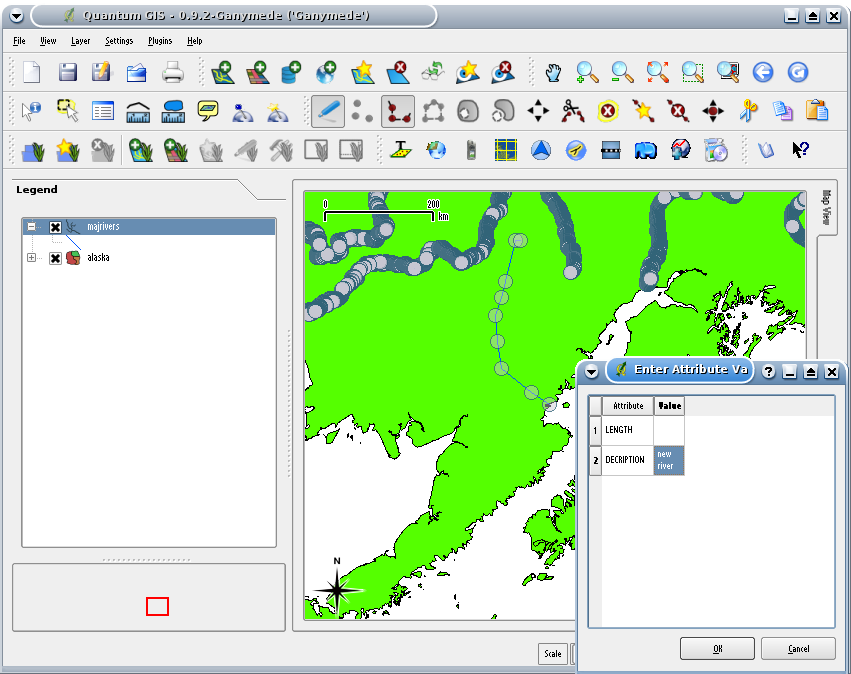
\includegraphics[clip=true, width=16cm]{digitising_attributes09}
\end{center}  
\end{figure}

\begin{Tip}[h]\caption{\textsc{Tipos de valores de atributos}}
\qgistip{En la versión actual de QGIS, la casilla del diálogo de atributos no comprueba si los datos introducidos concuerdan con el tipo esperado (ej.: numérico vs. texto). Asegúrese de esto antes de pulsar \textit{Aceptar}, de lo contrario puede encontrarse con que el error es detectado más tarde cuando intente guardar los cambios.
}
\end{Tip}

% These features will be added later
%
%\minisec{Move Selected Feature}
%\index{vector layers!move!feature}
%
%%% INPUT IS MISSING
%
%\minisec{Split Selected Feature}
%\index{vector layers!split!feature}
%
%%%% INPUT IS MISSING
%

\minisec{Editar vértices de un objeto espacial}
\index{vector layers!editing!vertex}

Se pueden editar los vértices de un objeto espacial, tanto para capas basadas en PostgreSQL/PostGIS como en archivos shape.

Los vértices se pueden editar directamente, esto es, no tiene que seleccionar el objeto espacial a editar antes de cambiar su geometría. En algunos casos, varios objetos espaciales pueden compartir el mismo vértice y entonces rigen las siguientes reglas cuando pulsa con el ratón cerca de los objetos espaciales del mapa:

\begin{itemize}
\item \textbf{Líneas}   - La línea más próxima a la posición del ratón se usa como el objeto espacial objetivo. Entonces (para mover y borrar un vértice) el vértice más 	                          próximo de esa línea será el objetivo de la edición.

\item \textbf{Polígonos} - Si el ratón está dentro de un polígono, entonces este será el objeto espacial objetivo; de lo contrario, se usará el polígono más próximo. Entonces (para mover y borrar un vértice) el vértice más próximo de ese polígono será el objetivo de la edición.
\end{itemize}

Necesitará establecer la propiedad \textit{Configuración}->\textit{Propiedades del proyecto}->\textit{General}->\textit{Tolerancia de autoensamblado} a un número mayor que cero. De lo contrario QGIS no será capaz de decir qué objeto espacial se está editando.


\minisec{Adñadir vértices a un objeto espacial}
\index{vector layers!adding!vertex}

Puede añadir nuevos vértices a un objeto espacial usando el icono \textit{Añadir vértice} de la barra de herramientas.

Nota: no tiene sentido añadir más vértices a objetos espaciales de tipo punto.

En esta versión de QGIS, los vértices sólo se pueden añadir a un segmento de línea \textit{existente} de un objeto espacial de tipo línea. Si quiere extender una línea más allá de su punto final, tendrá que mover primero el vértice final y luego añadir un nuevo vértice donde anteriormente se encontraba el final.

\minisec{Mover vértices de un objeto espacial}
\index{vector layers!moving!vertex}

Puede mover los vértices usando el icono \textit{Mover vértice} de la barra de herramientas.

\minisec{Borrar vértices de un objeto espacial}
\index{vector layers!deleting!vertex}

Puede borrar vértices usando el icono \textit{Borrar vértice} de la barra de herramientas.

Nota: no tiene sentido borrar el vértice de un objeto espacial de tipo punto. Borre la totalidad del objeto espacial en su lugar.

De forma similar, una línea con un solo vértice o un polígono con dos vértices son bastante inútiles y darán lugar a resultados inesperados en cualquier operación de QGIS, así que no los haga.

\textbf{Aviso:} un vértice se identifica para borrar en el momento que pulsa con el ratón cerca de un objeto espacial susceptible de ser borrado. Para deshacer, necesitará desactivar el modo de edición y descartar los cambios (por supuesto, esto implicará que cualquier otro cambio no guardado se pierda).

\minisec{Añadir anillos}
\index{vector layers!add!ring}
\textbf{Nuevo en v0.9}

Puede crear polígonos anulares en QGIS. Esto significa que dentro de un área existente es posible digitalizar más polígonos, lo que ocurrirá como un «todo», de forma que el área entre los límites de los polígonos exterior e interior quedará como un polígono anular.

\minisec{Añadir islas}
\index{vector layers!add!island}
\textbf{Nuevo en v0.9}

Puede añadir polígonos isla a un polígono múltiple seleccionado. El nuevo polígono isla tiene que digitalizarse fuera del polígono múltiple seleccionado.

% FIXME: In versions > 0.9.0 tries to convert a selected normal polygone to a
% multipolygone, if you try to use the "add island" funtionality. 
% (not yet implemented)

\minisec{Cortar, copiar y pegar objetos espaciales}
\index{vector layers!cut!feature}
\index{vector layers!copy!feature}
\index{vector layers!paste!feature}
\index{editing!cutting features}
\index{editing!copying features}
\index{editing!pasting features}

Se pueden cortar, copiar y pegar los objetos espaciales seleccionados entre capas dentro del mismo proyecto de QGIS, con tal de que las capas de destino se hayan puesto en modo edición con anterioridad.

Los objetos espaciales también se pueden pegar en aplicaciones externas como texto: esto es, los objetos espaciales se representan en formato CSV, apareciendo los datos de la geometría en formato OGC Well-Known Text (WKT).

Sin embargo, en esta versión de QGIS, los objetos espaciales de texto procedentes de fuera de QGIS no se pueden pegar en una capa dentro de QGIS.

¿Cuándo estarán disponibles las funciones de copiar y pegar? Bien, teniendo en cuenta que se puede editar más de una capa a la vez y copiar y pegar objetos espaciales entre ellas, ¿para qué querríamos hacer eso? Digamos que necesitamos trabajar en una nueva capa pero sólo necesitamos uno o dos lagos, no los 5.000 de nuestra capa \textsl{big\_lakes}. Podemos crear una nueva capa y usar copiar/pegar para añadirle los lagos que necesitemos.

Como ejemplo vamos a copiar algunos lagos a una capa nueva:

\begin{enumerate}
\item Cargar la capa de la que se quiere copiar (capa de origen).
\item Cargar o crear la capa en la que se quiere copiar (capa de destino).
\item Comenzar la edición de ambas capas.
\item Activar la capa origen pulsando en ella en la leyenda.
\item Usar la herramienta de selección para seleccionar los objetos espaciales de la capa de origen.
\item Pulsar en la herramienta \textsl{Copiar objetos espaciales}.
\item Activar la capa de destino pulsando en ella en la leyenda.
\item Pulsar en la herramienta \textsl{Pegar objetos espaciales}.
\item Detener la edición y guardar los cambios.
\end{enumerate}

¿Qué pasa si las capas de origen y destino tienen distintos esquemas (los nombres y tipos de campos no son iguales)? QGIS rellena lo que sea igual e ignora el resto. Si no le interesa que se copien los atributos en la capa de destino, no importa cómo diseñe los campos y el tipo de datos. Si quiere asegurarse de que todo, objetos espaciales y atributos, se copie, asegúrese de que los esquemas concuerdan.

\begin{Tip}[h]\caption{\textsc{Congruencia de los objetos espaciales pegados}}
\qgistip{Si sus capas de origen y destino usan la misma proyección, entonces los objetos espaciales tendrán pegados una geometría idéntica a la de la capa de origen. Sin embargo, si la capa de destino tiene una proyección diferente, QGIS no puede garantizar que la geometría sea idéntica. Esto es sencillamente porque hay pequeños errores de redondeo cuando se convierte entre proyecciones.
}
\end{Tip}

\minisec{Borrar objetos espaciales seleccionados}
\index{vector layers!deleting!feature}

Si quiere borrar un polígono entero, puede hacerlo seleccionando primero el polígono usando la herramienta habitual \textsl{Seleccionar objetos espaciales}. Puede seleccionar múltiples objetos espaciales para borrarlos. Una vez que tenga la selección, use la herramienta \textsl{Borrar lo seleccionado} para borrar los objetos espaciales. No existe una función deshacer, pero recuerde que su capa no cambia realmente hasta que detiene la edición y selecciona guardar los cambios. Por lo tanto, si comete un error, siempre puede cancelar el guardado.

La herramienta \textsl{Cortar objetos espaciales} de la barra de herramientas de digitalización también se puede usar para borrar objetos espaciales. Esto efectivamente borra el objeto espacial, pero lo coloca en un ``portapapeles espacial". Podemos entonces usar la herramienta pegar para restaurarlo, dándonos la capacidad de deshacer una acción. Cortar, copiar y pegar funcionan en los objetos espaciales actualmente seleccionados, lo que significa que podemos operar en más de uno a la vez.

\begin{Tip}[h]\caption{\textsc{Soporte para el borrado de objetos espaciales}}
\qgistip{Cuando se editan archivos shape de ESRI, el borrado de objetos espaciales sólo funciona si QGIS está enlazado a una versión de GDAL 1.3.2 o superior. Las versiones de QGIS para OS X y Window disponibles desde la página de descarga están compiladas usando GDAL 1.3.2 o superior.
}
\end{Tip}

\minisec{Modo de autoensamblado}
\index{editing!snap}
QGIS permite que los vértices digitalizados se ensamblen automáticamente a otros vértices de la misma capa. Para establecer la tolerancia de autoensamblado, vaya a \textit{Configuración}->\textit{Propiedades del proyecto}->\textit{General}->\textit{Tolerancia de autoensamblado}. Tenga en cuenta que la tolerancia de autoensamblado está en unidades de mapa.

\minisec{Guardar las capas editadas}
\index{editing!saving changes}

Cuando una capa está en modo edición, cualquier cambio permanece en la memoria de QGIS. Por lo tanto, no se transfieren/guardan de forma inmediata a la fuente de datos o al disco. Cuando desactiva el modo edición (o sale de QGIS para ello), se le pregunta si quiere guardar los cambios o descartarlos.

Si los cambios no se pueden guardar (por ejemplo, porque el disco este lleno o los atributos tienen valores que están fuera de intervalo), se conserva el estado de QGIS en memoria. Esto le permite ajustar sus ediciones y probar de nuevo.

\subsubsection{Crear una nueva capa}\label{sec:create shape}\index{editing!creating a new layer}

Para crear una capa nueva para editarla, seleccione \textit{Nueva capa vectorial...} del menú \textit{Capa}. El diálogo \textit{Nueva capa vectorial} se mostrará como aparece en la Figura \ref{fig:newvectorlayer}. Seleccione el tipo de capa (punto, línea o polígono).

\begin{figure}[ht]
   \begin{center}
   \caption{Diálogo de creación de un nuevo vectorial}\label{fig:newvectorlayer}\smallskip
   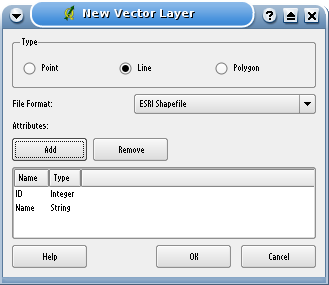
\includegraphics[clip=true, width=7cm]{newvectorlayer}
\end{center} 
\end{figure}

Nota: QGIS aún no tiene soporte para la creación de objetos espaciales 2.5D (esto es, objetos espaciales con coordenadas X, Y y Z). En este momento sólo se pueden crear archivos shape. En una versión futura de QGIS, estará soportada la creación de cualquier tipo de capa OGR o PostgreSQL. 

La creación de capas de GRASS es posible desde el complemento de GRASS. Por favor vaya a la sección \ref{sec:creating_new_grass_vectors} para más información sobre la creación de capas vectoriales de GRASS.

Para completar la creación de una nueva capa, añada los atributos que desee pulsando el botón \textit{Añadir} y especificando el nombre y tipo de atributos. Solo están soportados los atributos de tipo real, entero y cadera. Una vez que esté satisfecho con los atributos, pulse Aceptar y dele un nombre al archivo shape. QGIS añadirá automáticamente la extensión .shp al nombre que haya especificado. Una vez que la capa esté creada, se añadirá al mapa y la podrá editar de la misma forma descrita en la sección \ref{sec:edit_existing_layer} anterior.

\subsection{Constructor de consultas}\label{sec:query_builder}
\index{Query Builder}

El constructor de consultas le permite definir un subconjunto de una tabla y mostrarlo como una capa en QGIS. Se puede usar para todos los formatos soportados por OGR, archivos de GRASS y capas PostGIS. Por ejemplo, si tiene una capa de ciudades con un campo «población», podría seleccionar sólo las ciudades más grandes introduciendo \textsl{población > 100000} en el cuadro de consulta SQL del constructor de consultas. La Figura \ref{fig:query_builder} muestra un ejemplo del constructor de consultas relleno con datos de una capa PostGIS con atributos guardados en PostgreSQL.

\begin{figure}[ht]
  \begin{center}
    \caption{Constructor de consultas}\label{fig:query_builder}\smallskip
    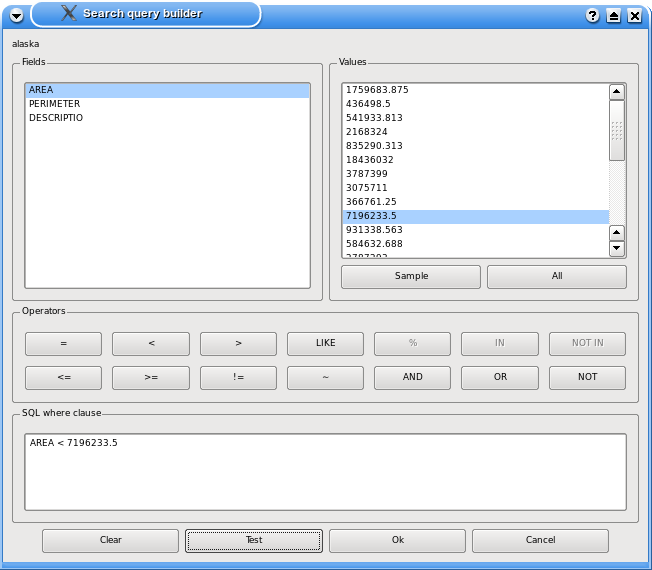
\includegraphics[clip=true, width=14cm]{querybuilder}
  \end{center}
\end{figure}

El constructor de consultas\index{Query Builder} muestra una lista de los campos que hay en la base de datos de la capa en el cuadro de lista de la izquierda. Puede obtener una muestra de los datos que contiene el campo resaltado pulsando en el botón \textit{Muestra}\index{Query Builder!generating sample list}. Esto recupera los primeros 25 valores distintos del campo de la base de datos. Para obtener una lista de todos los valores posibles de un campo, pulse en el botón \textit{Todos}\index{Query Builder!getting all values}. Para añadir un campo o valor seleccionado a la consulta, haga doble clic en él\index{Query Builder!adding fields}. Puede usar los distintos botones para construir la consulta o puede simplemente escribirla en el cuadro SQL.

Para probar una consulta, pulse en el botón \textit{Probar}\index{Query Builder!testing queries}. Esto devolverá la cuenta del número de registros que se incluirán en la capa. Cuando esté satisfecho con la consulta, pulse \textit{Aceptar}. La sentencia SQL para la cláusula «donde» se mostrará en la columna SQL de la lista de capas.

\begin{Tip}\caption{\textsc{Cambiar la definición de la capa}}\index{Query Builder!changing layer definitions} 
\qgistip{Puede cambiar la definición de la capa después de que esté cargada alterando la consulta SQL usada para definir la capa. Para hacer esto, abra el diálogo de propiedades de la capa vectorial haciendo doble clic en la capa en la leyenda y pulse el botón \textit{Constructor de consultas} en la pestaña \textit{General}. Vea la Sección 
\ref{sec:vectorprops} para más información.}
\end{Tip}

\subsubsection{Consultar capas PostGIS}\label{sec:query_builder_postgis}
\index{PostgreSQL!query builder}
\index{PostGIS!query builder}
\index{query builder!PostgreSQL}
\index{query builder!PostGIS}

Para consultar una capa PostGIS cargada hay dos opciones. La primera es pulsar en el botón \textit{Abrir tabla} para abrir la tabla de atributos de la capa PostGIS. Luego pulse el botón \textit{Avanzado...} en la parte inferior. Esto inicia el constructor de consultas que le permite definir un subconjunto de una tabla y mostrarlo como se describe en la Sección \ref{sec:query_builder}.

La segunda opción para consultar una capa PostGIS layer, es abrir el diálogo \textit{Propiedades de la capa} haciendo doble clic en el nombre de la capa PostGIS en la leyenda o clic derecho y seleccionar \textit{Propiedades} del menú emergente. En la pestaña \textit{General} pulse el botón \textit{Constructor de consultas} de la parte inferior.

\subsubsection{Consultar formatos OGR y archivos de GRASS}\label{sec:query_builder_ogrgrass}
\index{OGR!query builder}
\index{GRASS!query builder}
\index{query builder!OGR}
\index{query builder!GRASS}

Para consultar un archivo de GRASS cargado o un formato soportado por OGR actualmente necesita pulsar el botón \textit{Abrir tabla} para abrir la correspondiente tabla de atributos y pulsar el botón \textit{Avanzado...}. Esto inicia el constructor de consultas que le permite definir un subconjunto de una tabla y mostrarlo como se describe en la Sección \ref{sec:query_builder}. 

La segunda opción para iniciar el constructor de consultas descrita en la sección \ref{sec:query_builder_postgis} actualmente no está soportada para capas OGR y de GRASS.

\index{vector layers|)}